\section{Algoritmo del sistema centrale}
\subsection{Introduzione}
Se le unità viaggiano in modalità di guida automatica, il server centrale acquisisce un ruolo determinante nel comportamento dell'applicazione. Non essendo un \gls{attore}\textsubscript{G}, non vi sono \glspl{usecase}\textsubscript{G} ad esso attribuibili: si è quindi deciso di esplorarne il comportamento attraverso un diagramma di attività. Il diagramma propone un workflow ad alto livello che aiuta a delineare l'interazione del server centrale con le altre componenti del sistema

\subsection{Algoritmo per la gestione delle task}
%inserire immagine
%\begin{figure}[H]
%	\centering
%	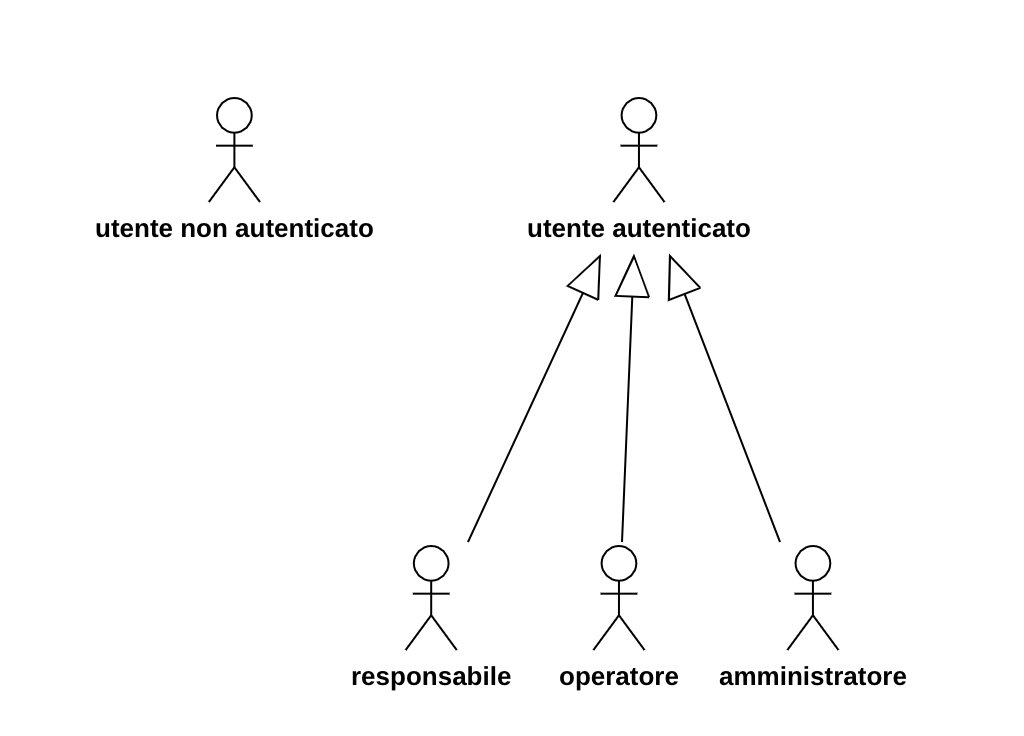
\includegraphics[scale=0.52]{res/images/gerarchia.png}
%	\caption{Attori primari}
%\end{figure}

\begin{itemize}
	\item{\textbf{INPUT}\\
	Il sistema centrale riceverà in input:
	\begin{itemize}
		\item{la mappa del magazzino}
		\item{la lista di unità disponibili}
		\item{le \gls{task}\textsubscript{G} da soddisfare, mano a mano che il responsabile le inserisce}
	\end{itemize}
	}
	\item{\textbf{OUTPUT}\\
	Il sistema allora dovrà:
	\begin{enumerate}
		\item{Suddividere le \gls{task}\textsubscript{G} in liste da assegnare alle unità nel punto di carico. \\
		Le liste sono calcolate suddividendo per zone di prossimità}
		\item{Per ogni unità \texttt{(while \glspl{task}\textsubscript{G}.length>0)}}
		\begin{enumerate}
			\item{viene calcolato il percorso ottimale per raggiungere il \acrshort{POI}\textsubscript{A} per soddisfare la prossima task}
			\item{viene suggerita la prossima mossa per raggiungere il \acrshort{POI}\textsubscript{A} della \gls{task}\textsubscript{G} \texttt{i}}	
			\begin{itemize}
				\item{\texttt{while(mosse.length > 0)}}
				\begin{itemize}
					\item{verifica fattibilità della mossa (es: unità in mezzo, ostacolo, corsia occupata, ingorgo)}
					\begin{itemize}
						\item{se la mossa è fattibile e se la gestione della guida è automatica =
						 attua la mossa}
						\item{altrimenti =
						ricalcolo del percorso a partire dalla mossa attuale}									\end{itemize}
				\end{itemize}				
				\item{attende la conferma dell'operatore che dichiara di aver eseguito lo scarico}
			\end{itemize}						
			\item{passa alla \gls{task}\textsubscript{G} successiva}				
		\end{enumerate}
		\item{Presenta un pulsante da cliccare se l'operatore ha finito il turno affinché lo riporti alla base. Se il pulsante non viene cliccato, esso viene portato al punto di carico. }
	\end{enumerate}
	}
\end{itemize}
\subsection{Diagramma di attività}
\begin{figure}[H]
	\centering
	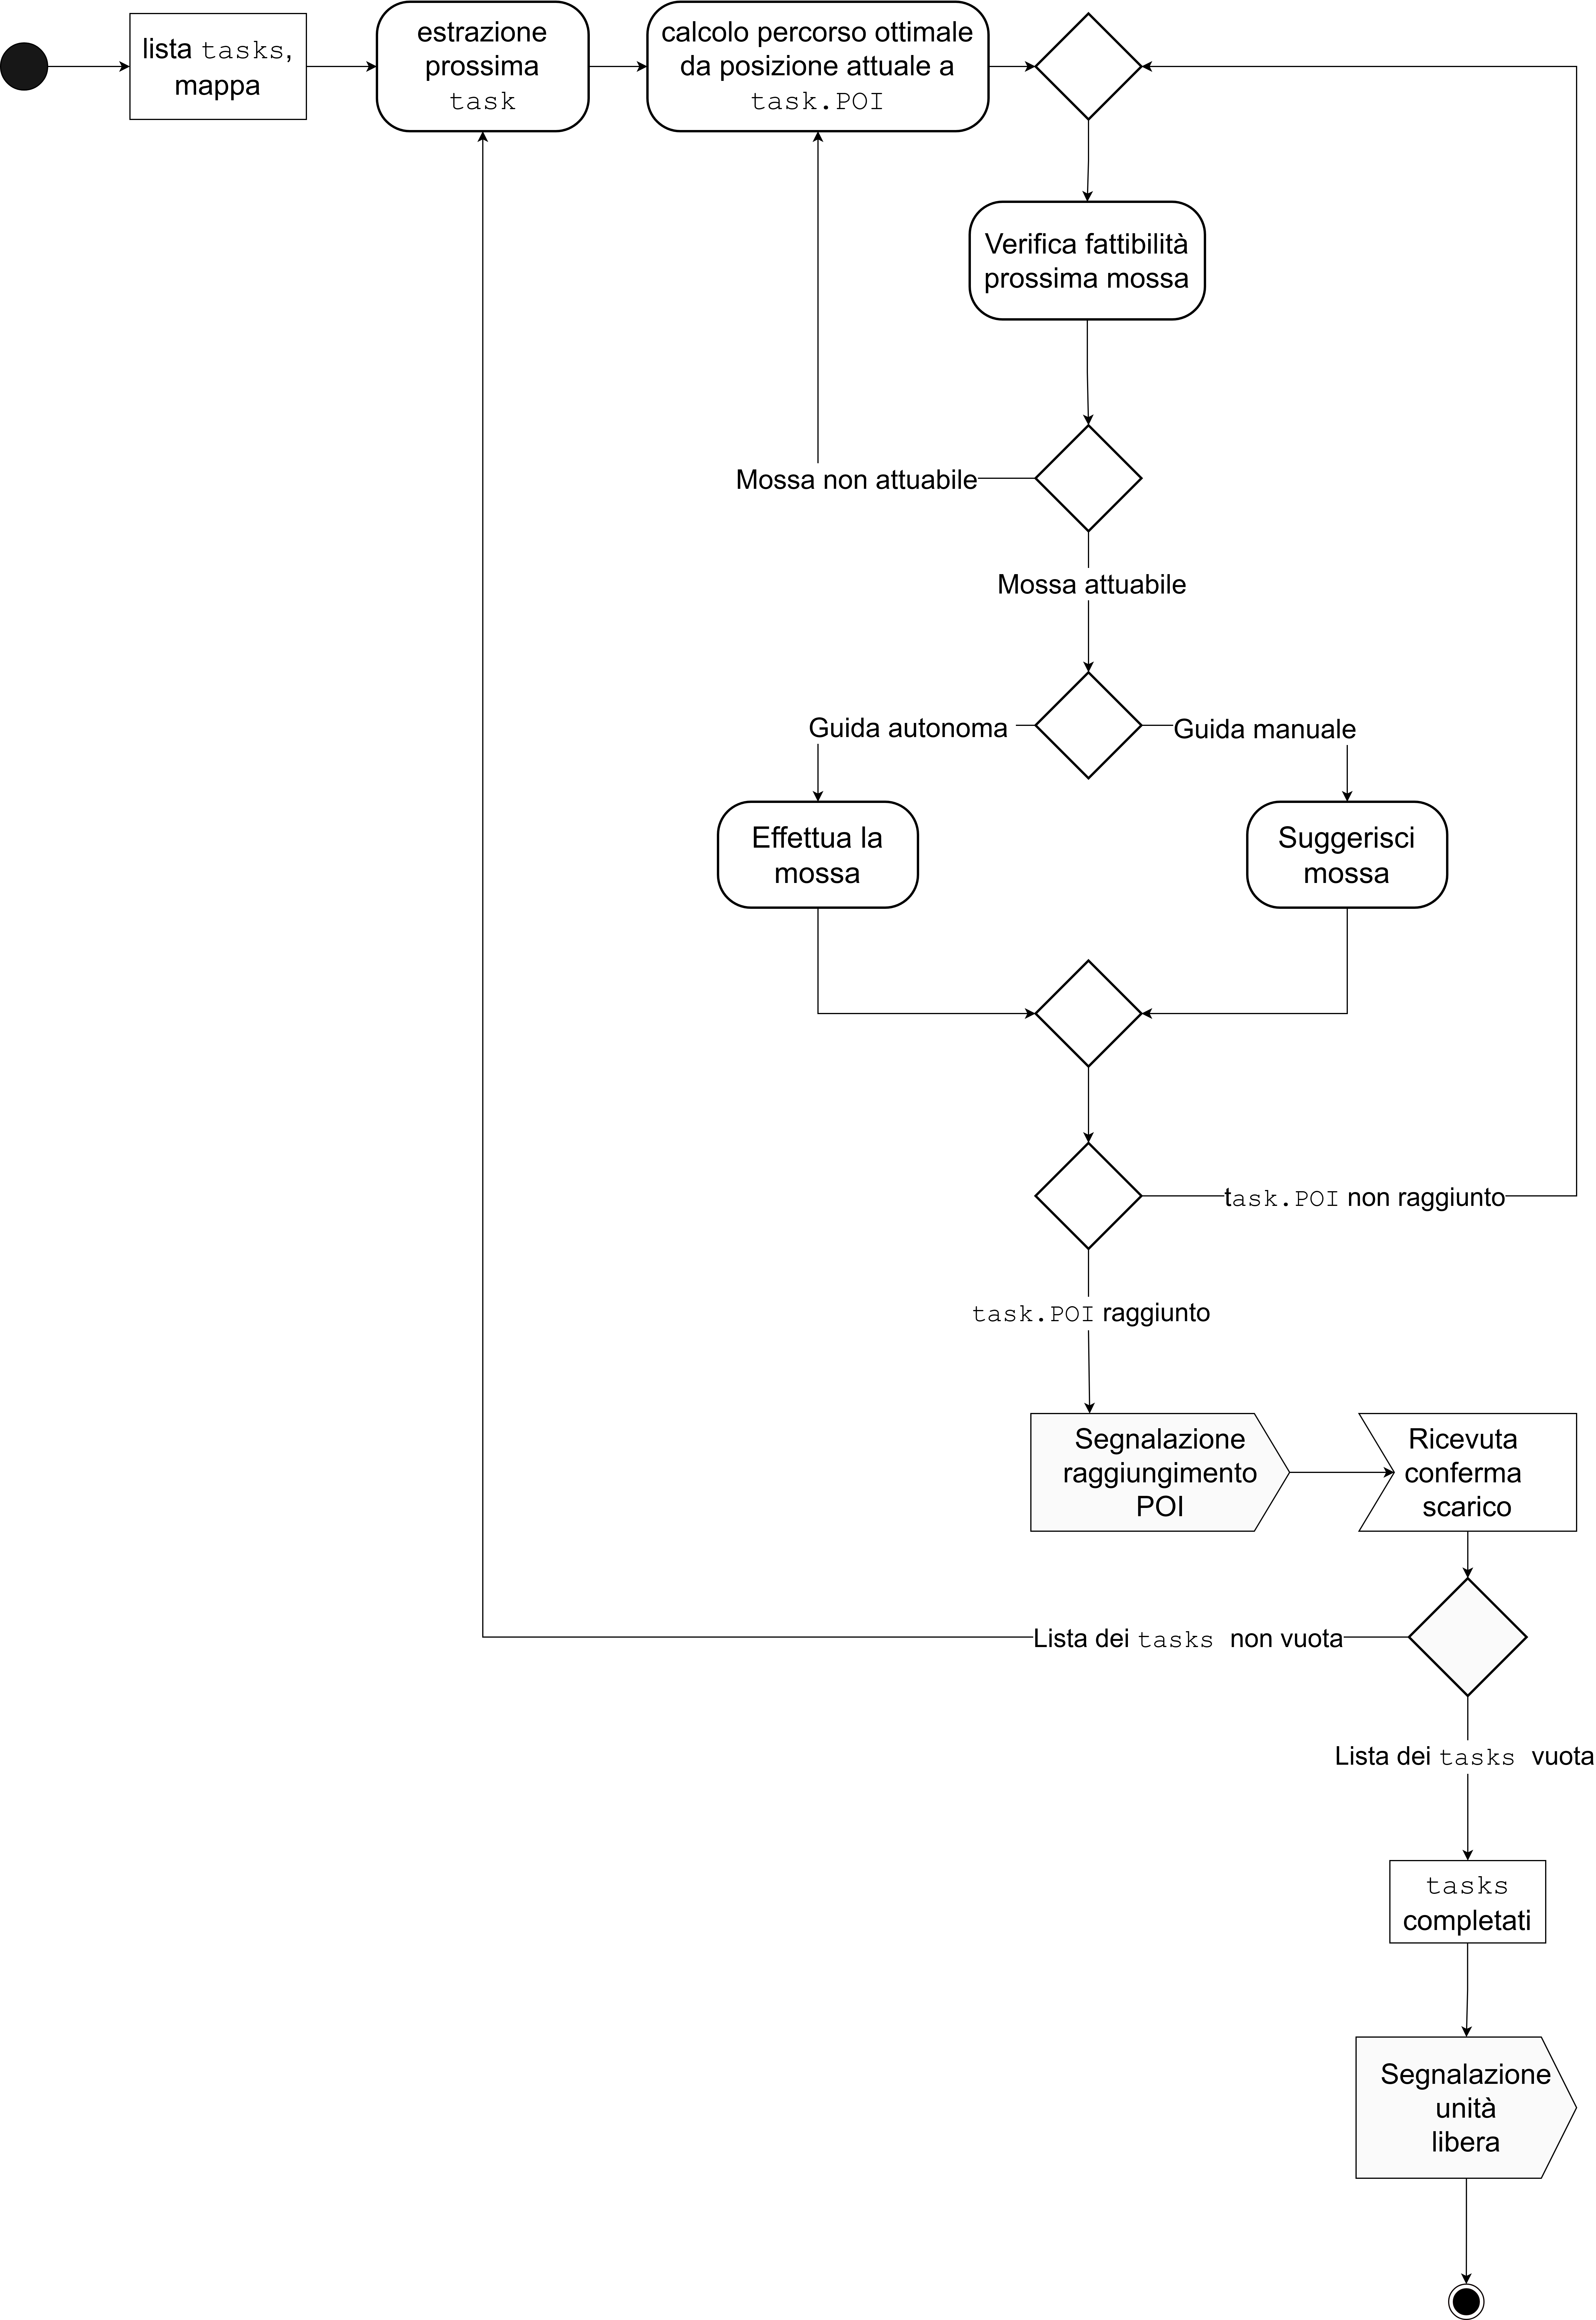
\includegraphics[scale=0.3]{res/images/diagramma_di_attivita2.png}
	\caption{Diagramma di attività per la gestione di una lista di task}
\end{figure}
\begin{figure}[H]
	\centering
	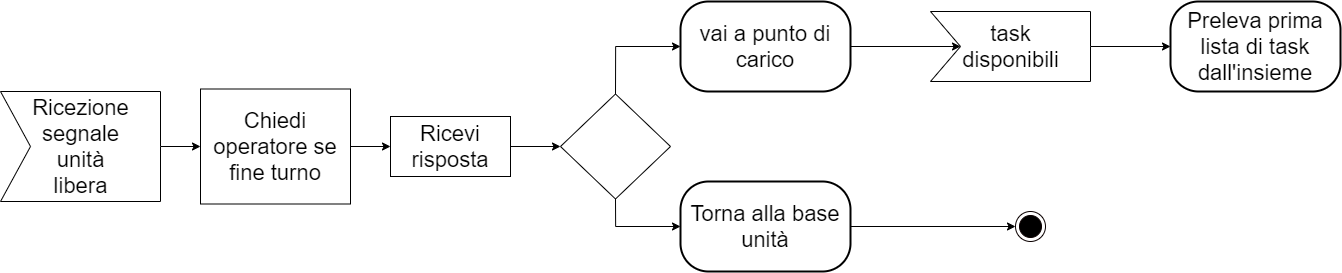
\includegraphics[scale=0.3]{res/images/diagramma_di_attivita1.png}
	\caption{Diagramma di attività per capire se tornare alla base o andare al punto di carico}
\end{figure}
\begin{figure}[H]
	\centering
	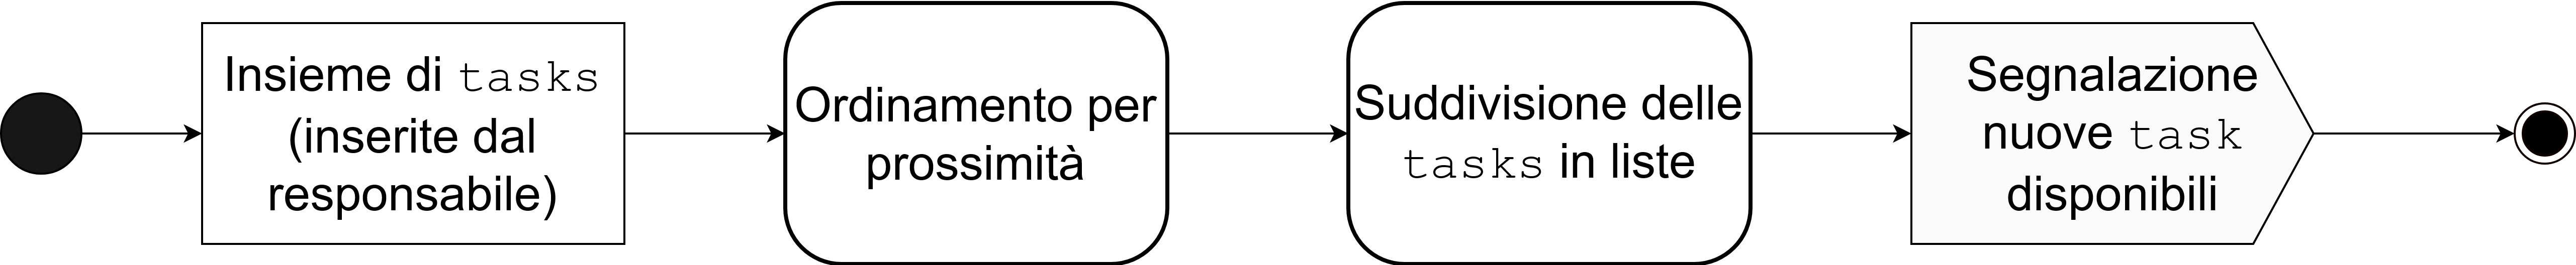
\includegraphics[scale=0.3]{res/images/diagramma_di_attivita3.png}
	\caption{Diagramma di attività per l'ordinamento lista delle task}
\end{figure}

